% !TEX root = main.tex

\textcolor{magenta}{\sout{Buildings are at the heart of society and currently account for 32\% of global final energy consumption and 19\% of energy related greenhouse gas emissions \cite{IPCC}. Nevertheless the building sector has a 50-90\% emission reduction potential using existing technologies, and widespread implementation could see energy use in buildings stabilise or even fall by 2050. Within this strategy, b}B}uilding integrated photovoltaics (BIPV) has the potential of providing a substantial segment of a buildings energy needs \cite{Shoen1997}. Even the photovoltaic (PV) industry has identified BIPV as one of the four key factors for the future success of PV \cite{raugei2009life}. \\

\textcolor{magenta}{\sout{The PV industry is currently dominated by crystaline silicon photovoltaic cells due to their high efficiency and low processing costs \cite{saga2010advances}. However these technologies are often difficult to integrate in a way that maintains the architectural expression of the building \cite{Lueling2009ee}. This combined with their intrinsic weight restricts their large scale implementation to roofs where they are out of sight. However, i}I}n the last decade, there has been interesting developments in second generation thin film technologies \cite{NREL}. In particular, Cu(In,Ga)Se$_2$ (CIGS) is reaching  competitive levels of efficiencies \cite{kushiya2014cis} and manufacturing costs \cite{kaelin2004low} \cite{jelle2012building}.\\

This development has brought new BIPV design possibilities. Their light weight nature and customisable shapes allows for easier and more aesthetically pleasing integration into the building envelope. Furthermore, this technology can be easily actuated and used as an adaptive building envelope\textcolor{magenta}{, because ...} \cite{rossi2012adaptive}. \\

Adaptive buildings envelopes have gained interest in recent years \textcolor{magenta}{\sout{due to their energy saving potentials} because they can be more easily integrated from a aestehtics point of view and because they come with the benefit of on-site energy production (\textit{How would they be "energy saving"?})} \cite{loonen2013climate}. \textcolor{magenta}{Traditionally the functional purpose of the building envelope, is to \sout{From an energetic perspective, the envelope}} act\textcolor{magenta}{\sout{s}} as a \textcolor{magenta}{\sout{buffer} barrier} between the interior and exterior environments. An adaptive building envelope can mediate solar isolation on the building, thereby offering reductions in heating/cooling loads and improvement of daylight distribution \cite{rossi2012adaptive}.

Interestingly the mechanics that actuate adaptive envelopes couples seamlessly with the mechanics required for facade integrated PV solar tracking. The balance of electricity production, and adaptive shading can in some cases offset the entire energy demand of an office space behind this adaptive envelope \cite{jayathissa2015abs}. We have proposed one possible combination of these technologies as the Adaptive Solar Facade (ASF).\textcolor{magenta}{\textit{Source?}}\\

\begin{figure}[H]
\begin{center}
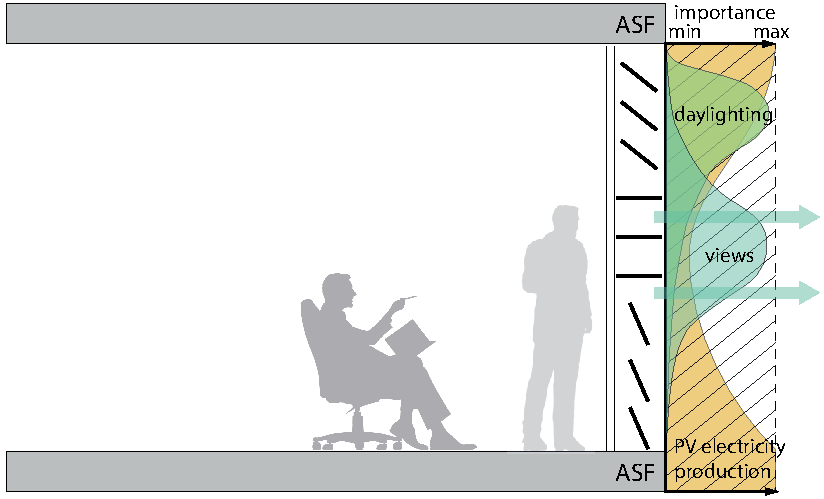
\includegraphics[width=8cm, trim= 0cm 0cm 0cm 0cm,clip]{facadeFunctions.pdf}
\caption{\textcolor{magenta}{\sout{The facade acting as a mediator between the interior and exterior environment, while fullfilling various functions \cite{nagy2015frontiers}}\textit{Delete IMHO}}}
\label{fig:ASFschematic}
\end{center}
\end{figure}

\begin{figure}[H]
\begin{center}
\includegraphics[width=8cm, trim= 0cm 0cm 0cm 0cm,clip]{honr.jpg}
\caption{Building Scale Prototype Constructed at the House of Natural Resources \cite{nagy2015frontiers}}
\label{fig:HoNR}
\end{center}
\end{figure}

The design of an ASF comes at an added cost. The additional electronics, actuators, and supporting structure adds further embodied CO2 to the product. It is therefore important to conduct a life cycle analysis (LCA) to analyse whether the carbon savings during operation offsets the increased embodied carbon emissions in manufacture\textcolor{magenta}{\textit{(This is the actually important message of the entire introduction, i.e. tradeoff material / benefit.)}}. It is also important to see how variations in design can alter the GHG reduction potential of the technology. Aspects such as the chosen PV material, actuator, and even location of operation can have a significant impact on its environmental performance. There has already been work conducted on static photovoltaic systems \cite{raugei2007life}, however this has not yet been expanded to adaptive BIPV systems. \\

In this paper we \textcolor{magenta}{\sout{will conduct an LCA of the ASF and determine which conditions, if at all, the ASF can truly provide an added benefit to GHG reductions.} investigate the aforementioned trade-off between added material and on-site energy production and other benefits (i.e. shading, etc.). To that end, we use the method of Life Cycle Impact Assessment (LCA). We assess a. the ASF system, b. the operation of a building, equipped by the ASF, and c. ...} \\

\textcolor{magenta}{\textit{(IMHO it is not really necessary to introduce each section beforehand.)}}In the next section we \textcolor{magenta}{\sout{will}} describe the inventory of the ASF and the LCA methodology used for analysing this adaptive system. In Section \ref{ch:results} we will present the results from the LCA and look at the major sources of embodied carbon, along with the operational performance. In this section we will also compare the results of the LCA with other technologies and its performance in different regions. In Section \ref{ch:discussion} we discuss the results and provide design recommendations for future adaptive building integrated photovoltaic installations. 






% - In the last decades, building integrated photovoltaics (BIPV) have been adopted as part of the energy strategy towards 2050... \

% (advantages of BIPV, potential of BIPV)\\


% - The current developments of light-weight efficient thin film technologies have brought new design possibilities for architects in BIPV design... \

% (Adaptive Building Envelopes, examples, Envelope is the barrier between the internal and external environment, Advantages, seamless coupling with solar tracking mechanics) \\

% - One example of a multi functional facade that was recently released is the Adaptive Solar Facade.\\

% - The aim of this paper is to analyse the life cycle emissions of an adaptive solar facade and provide comparisons with standard shading systems and static BIPV solutions.\\
